\documentclass[11pt,a4paper]{article}

% Packages
\usepackage{amsmath}
\usepackage{amssymb}
\usepackage{amsthm}
\usepackage[margin=1in]{geometry}
\usepackage{enumitem}
\usepackage{tikz}
\usepackage{pgfplots}
\usepackage{xcolor}
\pgfplotsset{compat=1.18}

% Custom commands
\newcommand{\stage}[1]{\textbf{\textcolor{blue}{#1}}}

% Title information
\title{Exercise Sheet 3: Bifurcations\\
Question 2 - Complete Solution}
\author{Methods of Applied Mathematics}
\date{}

\begin{document}

\maketitle

\section*{Problem Statement}

Consider the system:
\[
\dot{x} = a + 2x + x^2
\]

\textbf{Tasks:}
\begin{enumerate}[label=(\alph*)]
\item Find the equilibria of the system and their stability
\item Conjecture the bifurcation that occurs in the system
\item Evaluate the bifurcation and genericity conditions to prove your conjecture
\end{enumerate}

\vspace{10pt}
\hrule
\vspace{10pt}

\section{Step 1: Find Equilibria}

\subsection*{Set up equilibrium condition}

For equilibria, we require $\dot{x} = 0$:
\[
a + 2x + x^2 = 0
\]

Rearranging as standard quadratic:
\[
x^2 + 2x + a = 0
\]

\subsection*{Apply quadratic formula}

\[
x = \frac{-2 \pm \sqrt{4 - 4a}}{2} = \frac{-2 \pm 2\sqrt{1-a}}{2} = -1 \pm \sqrt{1-a}
\]

\subsection*{Analyze discriminant}

The discriminant is $\Delta = 4(1-a)$. The number of real equilibria depends on its sign:

\begin{align*}
a < 1: \quad & \Delta > 0 \quad \Rightarrow \quad \text{Two distinct real equilibria:} \\
& \boxed{x_+^* = -1 + \sqrt{1-a}} \quad \text{and} \quad \boxed{x_-^* = -1 - \sqrt{1-a}} \\[10pt]
a = 1: \quad & \Delta = 0 \quad \Rightarrow \quad \text{One repeated equilibrium:} \\
& \boxed{x^* = -1} \\[10pt]
a > 1: \quad & \Delta < 0 \quad \Rightarrow \quad \text{No real equilibria}
\end{align*}

\subsection*{XYZ Analysis of Equilibrium Structure}

\begin{itemize}[leftmargin=*]
\item \stage{STAGE X (What we found):} The number of equilibria changes as parameter $a$ varies: two for $a<1$, one for $a=1$, zero for $a>1$.

\item \stage{STAGE Y (Why this happens):} The equation $x^2 + 2x + a = 0$ represents the intersection of parabola $y = x^2 + 2x$ (opening upward, vertex at $x=-1, y=-1$) with horizontal line $y = -a$:
\begin{itemize}
\item For $a < 1$: Line $y = -a$ is above $y = -1$ (vertex), intersecting parabola twice
\item For $a = 1$: Line $y = -1$ touches parabola at vertex (tangent)
\item For $a > 1$: Line $y = -a$ is below vertex, missing parabola entirely
\end{itemize}
As $a$ increases through 1, two equilibria approach each other along the $x$-axis, collide at $x=-1$, then disappear into the complex plane.

\item \stage{STAGE Z (What this means):} Equilibria are created/destroyed at $a=1$, suggesting a fold (saddle-node) bifurcation. Unlike transcritical (where equilibria pass through each other), here they annihilate.
\end{itemize}

\vspace{10pt}
\hrule
\vspace{10pt}

\section{Step 2: Determine Stability}

\subsection*{Compute derivative}

For $f(x) = a + 2x + x^2$:
\[
f'(x) = 2 + 2x
\]

\subsection*{Evaluate at each equilibrium}

\textbf{At $x_+^* = -1 + \sqrt{1-a}$:}
\begin{align*}
f'(x_+^*) &= 2 + 2(-1 + \sqrt{1-a}) \\
&= 2 - 2 + 2\sqrt{1-a} \\
&= 2\sqrt{1-a}
\end{align*}

For $a < 1$: $\sqrt{1-a} > 0$, so $f'(x_+^*) = 2\sqrt{1-a} > 0$

\[
\boxed{\text{UNSTABLE}}
\]

\textbf{At $x_-^* = -1 - \sqrt{1-a}$:}
\begin{align*}
f'(x_-^*) &= 2 + 2(-1 - \sqrt{1-a}) \\
&= 2 - 2 - 2\sqrt{1-a} \\
&= -2\sqrt{1-a}
\end{align*}

For $a < 1$: $\sqrt{1-a} > 0$, so $f'(x_-^*) = -2\sqrt{1-a} < 0$

\[
\boxed{\text{STABLE}}
\]

\textbf{At $a = 1$ (critical point $x^* = -1$):}
\[
f'(-1) = 2 + 2(-1) = 0 \quad \Rightarrow \quad \boxed{\text{NEUTRAL}}
\]

\subsection*{Stability summary}

\begin{center}
\begin{tabular}{|c|c|c|}
\hline
\textbf{Parameter} & \textbf{Equilibrium} & \textbf{Stability} \\
\hline
\multirow{2}{*}{$a < 1$} & $x_+^* = -1 + \sqrt{1-a}$ & Unstable \\
\cline{2-3}
& $x_-^* = -1 - \sqrt{1-a}$ & Stable \\
\hline
$a = 1$ & $x^* = -1$ & Neutral \\
\hline
$a > 1$ & None & --- \\
\hline
\end{tabular}
\end{center}

\subsection*{XYZ Analysis of Stability}

\begin{itemize}[leftmargin=*]
\item \stage{STAGE X (What we found):} For $a<1$, the right equilibrium ($x_+^*$, closer to zero) is unstable, the left equilibrium ($x_-^*$, more negative) is stable. At $a=1$, both collapse to a neutral equilibrium.

\item \stage{STAGE Y (Why these stabilities):} The derivative $f'(x) = 2 + 2x$ is a linear function of $x$:
\begin{itemize}
\item $f'(x) > 0$ for $x > -1$ (right of critical point) $\Rightarrow$ unstable
\item $f'(x) < 0$ for $x < -1$ (left of critical point) $\Rightarrow$ stable
\item $f'(x) = 0$ at $x = -1$ (the critical point) $\Rightarrow$ neutral
\end{itemize}
Since $x_+^* = -1 + \sqrt{1-a} > -1$ (always to the right), it's unstable. Since $x_-^* = -1 - \sqrt{1-a} < -1$ (always to the left), it's stable. As $a \to 1^-$, both approach $x=-1$ from opposite sides, maintaining their stabilities until they meet.

\item \stage{STAGE Z (What this means):} A stable and unstable equilibrium collide at $a=1$. This is the characteristic signature of a fold/saddle-node bifurcation: one equilibrium attracts, one repels, they meet and mutually annihilate. No stability exchange occurs (contrast with transcritical).
\end{itemize}

\vspace{10pt}
\hrule
\vspace{10pt}

\section{Step 3: Conjecture Bifurcation Type}

\subsection*{Observed features}

From our analysis:
\begin{enumerate}
\item Two equilibria exist for $a < 1$
\item Equilibria collide at $a = 1$, $x = -1$
\item No equilibria exist for $a > 1$
\item One equilibrium is stable, one unstable before collision
\item At collision point, derivative is zero: $f'(-1) = 0$
\end{enumerate}

\subsection*{Conjecture}

\[
\boxed{\text{FOLD BIFURCATION (also called SADDLE-NODE BIFURCATION)}}
\]
occurs at $(a, x) = (1, -1)$.

\subsection*{XYZ Analysis of Bifurcation Conjecture}

\begin{itemize}[leftmargin=*]
\item \stage{STAGE X (What we observe):} Equilibria are created/destroyed (not exchanged or multiplied). Number changes from 2 to 0 across the bifurcation.

\item \stage{STAGE Y (Why fold specifically):} The distinguishing features match fold bifurcation:
\begin{itemize}
\item \textbf{Creation/annihilation}: Equilibria appear from nowhere (for decreasing $a$) or disappear into complex plane (for increasing $a$)
\item \textbf{Pairing}: A stable-unstable pair collides (in higher dimensions, typically a saddle and node, hence "saddle-node")
\item \textbf{Tangency}: At bifurcation, $f'=0$ and the equilibrium is tangent to the $a$-axis in $(a,x)$ space
\item \textbf{Generic}: No special symmetry required (unlike pitchfork) and no pinned equilibrium (unlike transcritical)
\end{itemize}
This is \textit{not} transcritical because equilibria don't pass through each other - they vanish. It's \textit{not} pitchfork because only two equilibria are involved (not one splitting into three) and there's no symmetry $f(x) = f(-x)$.

\item \stage{STAGE Z (What this means):} The fold is the most common codimension-1 bifurcation in generic systems. It represents a threshold phenomenon: for $a>1$, the system has no steady states and diverges; for $a<1$, steady behavior is possible. The critical value $a=1$ is the "tipping point."
\end{itemize}

\vspace{10pt}
\hrule
\vspace{10pt}

\section{Step 4: Verify Bifurcation Conditions}

\subsection*{Fold bifurcation requirements}

From lecture notes (Section 13, pages 46-47), a fold bifurcation at $(a^*, x^*)$ requires:

\textbf{Bifurcation conditions:}
\begin{itemize}
\item[(B1)] $f(x^*, a^*) = 0$ \quad (equilibrium exists)
\item[(B2)] $\frac{\partial f}{\partial x}\bigg|_{(x^*, a^*)} = 0$ \quad (zero eigenvalue)
\end{itemize}

\textbf{Genericity conditions:}
\begin{itemize}
\item[(G1)] $\frac{\partial^2 f}{\partial x^2}\bigg|_{(x^*, a^*)} \neq 0$ \quad (second derivative nonzero)
\item[(G2)] $\frac{\partial f}{\partial a}\bigg|_{(x^*, a^*)} \neq 0$ \quad (positive speed of $f$ in $a$)
\end{itemize}

\subsection*{Check conditions at $(a, x) = (1, -1)$}

For $f(x, a) = a + 2x + x^2$:

\textbf{(B1) Equilibrium condition:}
\[
f(-1, 1) = 1 + 2(-1) + (-1)^2 = 1 - 2 + 1 = 0 \quad \checkmark
\]

\textbf{(B2) Zero eigenvalue:}
\[
\frac{\partial f}{\partial x} = 2 + 2x \quad \Rightarrow \quad \frac{\partial f}{\partial x}\bigg|_{x=-1} = 2 + 2(-1) = 0 \quad \checkmark
\]

\textbf{(G1) Second derivative nonzero:}
\[
\frac{\partial^2 f}{\partial x^2} = 2 \quad \Rightarrow \quad \frac{\partial^2 f}{\partial x^2}\bigg|_{(1,-1)} = 2 \neq 0 \quad \checkmark
\]

\textbf{(G2) Parameter derivative nonzero:}
\[
\frac{\partial f}{\partial a} = 1 \quad \Rightarrow \quad \frac{\partial f}{\partial a}\bigg|_{(1,-1)} = 1 \neq 0 \quad \checkmark
\]

\subsection*{Conclusion}

All four conditions satisfied:
\[
\boxed{\text{FOLD BIFURCATION CONFIRMED at } (a, x) = (1, -1)}
\]

\subsection*{XYZ Analysis of Condition Verification}

\begin{itemize}[leftmargin=*]
\item \stage{STAGE X (What we verified):} All bifurcation conditions (B1-B2) and genericity conditions (G1-G2) hold at the critical point.

\item \stage{STAGE Y (Why each condition matters):}
\begin{itemize}
\item \textbf{(B1) $f=0$}: Fundamental requirement - we need an equilibrium at the bifurcation point
\item \textbf{(B2) $f'=0$}: The linearization has zero eigenvalue, meaning we can't determine stability from linear terms alone. This is the algebraic signature of equilibria colliding - both have the same derivative value
\item \textbf{(G1) $f'' \neq 0$}: Ensures the nonlinearity is "strong enough" to create the fold. If $f''=0$ too, we'd have a higher-order (degenerate) bifurcation like a cusp. Here $f''=2>0$ means the parabola opens upward
\item \textbf{(G2) $\partial f/\partial a \neq 0$}: Ensures equilibrium positions actually change with parameter $a$. If this were zero, varying $a$ wouldn't move the equilibria, and no bifurcation would occur. Here $\partial f/\partial a = 1 > 0$ means increasing $a$ shifts $f$ upward, pushing equilibria together
\end{itemize}

\item \stage{STAGE Z (What this rigor provides):} These conditions aren't just a checklist - they guarantee the system near $(1,-1)$ can be transformed to the normal form $\dot{y} = \mu + y^2$ (or $\mu - y^2$ depending on sign of $f''$). This universality means our local analysis captures the essential behavior shared by all fold bifurcations.
\end{itemize}

\vspace{10pt}
\hrule
\vspace{10pt}

\section{Step 5: Normal Form Connection}

\subsection*{Standard fold normal form}

The canonical form is:
\[
\dot{y} = \mu \pm y^2
\]

where $\mu$ is the bifurcation parameter near zero.

\subsection*{Transform to normal form}

Let's verify our system near $(a,x) = (1,-1)$ matches this structure.

Define shifted coordinates:
\begin{align*}
\mu &= a - 1 \quad \text{(bifurcation parameter, zero at critical point)} \\
y &= x + 1 \quad \text{(spatial coordinate, zero at critical equilibrium)}
\end{align*}

Then $a = \mu + 1$ and $x = y - 1$. Substitute into $\dot{x} = a + 2x + x^2$:
\begin{align*}
\dot{y} &= \dot{x} = a + 2x + x^2 \\
&= (\mu + 1) + 2(y-1) + (y-1)^2 \\
&= \mu + 1 + 2y - 2 + y^2 - 2y + 1 \\
&= \mu + y^2
\end{align*}

Therefore:
\[
\boxed{\dot{y} = \mu + y^2}
\]

This is precisely the fold bifurcation normal form with the "$+$" sign (since $f'' = 2 > 0$).

\subsection*{XYZ Analysis of Normal Form}

\begin{itemize}[leftmargin=*]
\item \stage{STAGE X (What we derived):} Through coordinate shift $(a,x) \to (\mu, y)$ centered at the bifurcation point, our equation reduces exactly to the standard form $\dot{y} = \mu + y^2$ with no higher-order terms needed.

\item \stage{STAGE Y (Why this works):} The Taylor expansion of $f(x,a)$ around $(1,-1)$ is:
\[
f(x,a) = \underbrace{f(-1,1)}_{=0} + \underbrace{f_x(-1,1)}_{=0} (x+1) + \underbrace{f_a(-1,1)}_{=1}(a-1) + \frac{1}{2}\underbrace{f_{xx}(-1,1)}_{=2}(x+1)^2 + \cdots
\]
The linear term in $x$ vanishes (condition B2), leaving only the parameter term and quadratic term - exactly the normal form structure. Higher-order terms ($y^3$, $\mu y$, etc.) are genuinely absent because our $f$ is only quadratic in $x$ and linear in $a$.

\item \stage{STAGE Z (What this means):} The normal form isn't just an approximation for our system - it's exact. This makes our analysis particularly clean. For general systems, we'd have $\dot{y} = \mu + y^2 + O(|y|^3, |y||\mu|)$, but the qualitative behavior (equilibria colliding along a square-root curve) would be the same.
\end{itemize}

\vspace{10pt}
\hrule
\vspace{10pt}

\section{Step 6: Bifurcation Diagram}

\subsection*{Equilibrium curves in $(a,x)$ space}

From $x = -1 \pm \sqrt{1-a}$, the equilibria trace out curves:

\textbf{Upper branch:} $x_+(a) = -1 + \sqrt{1-a}$ (unstable, dashed)
\begin{itemize}
\item Exists for $a \leq 1$
\item At $a = 1$: $x_+ = -1$
\item As $a \to -\infty$: $x_+ \to +\infty$
\item As $a \to 1^-$: $x_+ \to -1$ (approaches bifurcation from right)
\end{itemize}

\textbf{Lower branch:} $x_-(a) = -1 - \sqrt{1-a}$ (stable, solid)
\begin{itemize}
\item Exists for $a \leq 1$
\item At $a = 1$: $x_- = -1$
\item As $a \to -\infty$: $x_- \to -\infty$
\item As $a \to 1^-$: $x_- \to -1$ (approaches bifurcation from left)
\end{itemize}

\subsection*{Bifurcation diagram}

\begin{center}
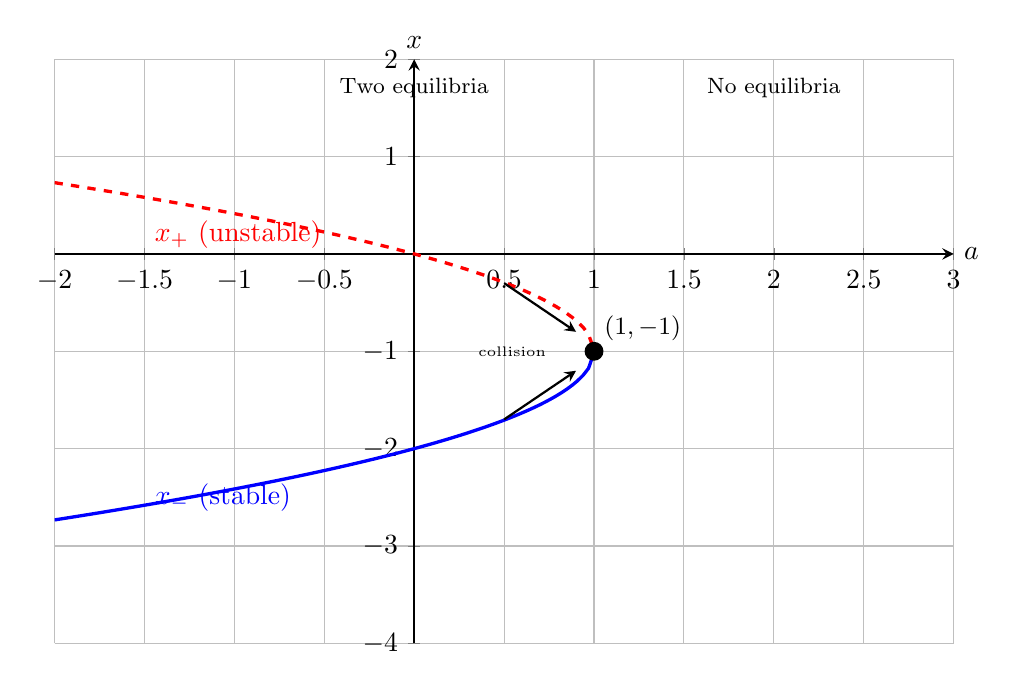
\begin{tikzpicture}
\begin{axis}[
    width=13cm,
    height=9cm,
    xlabel={$a$},
    ylabel={$x$},
    xmin=-2, xmax=3,
    ymin=-4, ymax=2,
    grid=major,
    axis lines=middle,
    thick,
    every axis x label/.style={at={(current axis.right of origin)},anchor=west},
    every axis y label/.style={at={(current axis.above origin)},anchor=south}
]

% Upper branch (unstable)
\addplot[red, very thick, dashed, domain=-2:1, samples=100] {-1 + sqrt(1-x)};

% Lower branch (stable)
\addplot[blue, very thick, solid, domain=-2:1, samples=100] {-1 - sqrt(1-x)};

% Bifurcation point
\addplot[mark=*, mark size=3pt, black, only marks] coordinates {(1, -1)};
\node[above right, font=\small] at (axis cs:1,-1) {$(1, -1)$};

% Labels
\node[red, anchor=west] at (axis cs:-1.5,0.2) {$x_+$ (unstable)};
\node[blue, anchor=west] at (axis cs:-1.5,-2.5) {$x_-$ (stable)};

% Regions
\node[font=\footnotesize, anchor=south] at (axis cs:0,1.5) {Two equilibria};
\node[font=\footnotesize, anchor=south] at (axis cs:2,1.5) {No equilibria};

% Arrow indicating collision
\draw[thick, ->, >=stealth] (axis cs:0.5,-0.3) -- (axis cs:0.9,-0.8);
\draw[thick, ->, >=stealth] (axis cs:0.5,-1.7) -- (axis cs:0.9,-1.2);
\node[font=\tiny, anchor=west] at (axis cs:0.3,-1) {collision};

\end{axis}
\end{tikzpicture}
\end{center}

\subsection*{XYZ Analysis of Bifurcation Diagram}

\begin{itemize}[leftmargin=*]
\item \stage{STAGE X (What the diagram shows):} Two parabolic branches meeting at $(1,-1)$ like a "fold" in the $(a,x)$ plane. The branches exist only for $a \leq 1$ and terminate at the bifurcation point. For $a > 1$, no branches exist - no real equilibria.

\item \stage{STAGE Y (Why this shape):} The equilibrium equation $x^2 + 2x + a = 0$ can be rearranged as:
\[
a = -x^2 - 2x = -(x+1)^2 + 1
\]
This is a parabola in $(a,x)$ space, opening leftward, with vertex at $(a,x) = (1,-1)$. Each horizontal line $a = \text{const}$ intersects this parabola:
\begin{itemize}
\item Twice if $a < 1$ (line to left of vertex) $\Rightarrow$ two equilibria
\item Once if $a = 1$ (line through vertex) $\Rightarrow$ one equilibrium
\item Not at all if $a > 1$ (line to right of vertex) $\Rightarrow$ no equilibria
\end{itemize}
The square-root dependence $x \propto \pm\sqrt{1-a}$ near $a=1$ is universal to fold bifurcations - equilibria approach the critical point along two branches that are tangent to each other (both have infinite slope $dx/da$ at $a=1$).

\item \stage{STAGE Z (What this means dynamically):} As $a$ increases:
\begin{itemize}
\item For $a \ll 1$: Two well-separated equilibria; stable one far left attracts trajectories
\item As $a \to 1^-$: Equilibria approach; stable attractor moves right toward $x=-1$
\item At $a = 1$: Equilibria merge; system at critical point
\item For $a > 1$: No equilibria exist; system has no steady state, $\dot{x} = a + 2x + x^2 > 0$ for all $x$ when $a>1$ and $x$ near $-1$, so solutions diverge to $+\infty$
\end{itemize}
This represents a catastrophic transition: beyond $a=1$, stable behavior is impossible.
\end{itemize}

\vspace{10pt}
\hrule
\vspace{10pt}

\section{Step 7: Phase Portraits}

\subsection*{Three scenarios}

\begin{center}
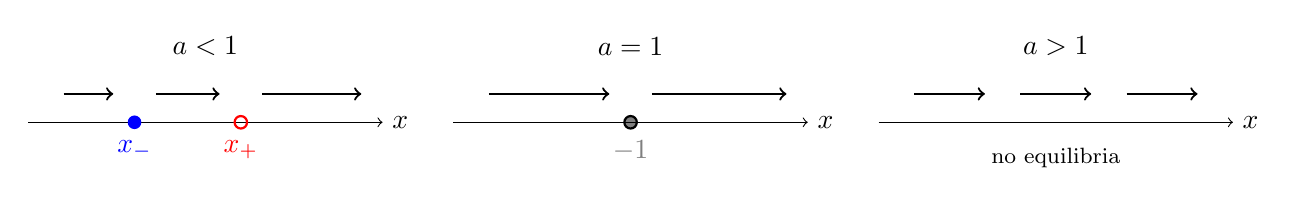
\begin{tikzpicture}[scale=0.9]
% a < 1
\begin{scope}
\draw[->] (-1,0) -- (4,0) node[right] {$x$};
\node[above] at (1.5,0.8) {$a < 1$};
% Stable at x_-
\filldraw[blue] (0.5,0) circle (2.5pt) node[below=3pt] {$x_-$};
% Unstable at x_+
\draw[red, thick] (2,0) circle (2.5pt) node[below=3pt] {$x_+$};
% Flow arrows
\draw[->, thick] (-0.5,0.4) -- (0.2,0.4);
\draw[->, thick] (0.8,0.4) -- (1.7,0.4);
\draw[->, thick] (2.3,0.4) -- (3.7,0.4);
\end{scope}

% a = 1
\begin{scope}[shift={(6,0)}]
\draw[->] (-1,0) -- (4,0) node[right] {$x$};
\node[above] at (1.5,0.8) {$a = 1$};
% Half-stable at x=-1
\draw[black, thick, fill=black, fill opacity=0.5] (1.5,0) circle (2.5pt) node[below=3pt] {$-1$};
% Flow arrows
\draw[->, thick] (-0.5,0.4) -- (1.2,0.4);
\draw[->, thick] (1.8,0.4) -- (3.7,0.4);
\end{scope}

% a > 1
\begin{scope}[shift={(12,0)}]
\draw[->] (-1,0) -- (4,0) node[right] {$x$};
\node[above] at (1.5,0.8) {$a > 1$};
% No equilibria - all arrows right
\draw[->, thick] (-0.5,0.4) -- (0.5,0.4);
\draw[->, thick] (1,0.4) -- (2,0.4);
\draw[->, thick] (2.5,0.4) -- (3.5,0.4);
\node[font=\footnotesize] at (1.5,-0.5) {no equilibria};
\end{scope}
\end{tikzpicture}
\end{center}

\textit{Notation: Filled circle = stable, hollow circle = unstable, half-filled = half-stable}

\subsection*{XYZ Analysis of Phase Portrait Evolution}

\begin{itemize}[leftmargin=*]
\item \stage{STAGE X (What we see):} Three qualitatively different flow patterns. Before bifurcation: two equilibria with flows toward stable one. At bifurcation: one half-stable equilibrium (attracts from left, repels to right). After bifurcation: no equilibria, all trajectories escape to infinity.

\item \stage{STAGE Y (Why these dynamics):} The sign of $\dot{x} = a + 2x + x^2$ determines flow direction:
\begin{itemize}
\item \textbf{For $a < 1$}: Between equilibria $x_- < x < x_+$, we have $\dot{x} = a + 2x + x^2 < 0$ because the parabola $x^2+2x$ is below $-a$ in this interval. Flow is leftward toward $x_-$. Outside the equilibria, flow is rightward ($x < x_-$) or rightward ($x > x_+$).
\item \textbf{For $a = 1$}: At $x = -1$, $\dot{x} = 0$. For $x < -1$, $\dot{x} < 0$ (leftward), for $x > -1$, $\dot{x} > 0$ (rightward). The equilibrium is "half-stable" - stable from left, unstable to right.
\item \textbf{For $a > 1$}: No equilibria exist. For $x$ near where they used to be (around $x=-1$), we have $\dot{x} = a + 2x + x^2 \approx 1 + 2x + x^2 = (x+1)^2 > 0$ for $x \neq -1$. Since the parabola has no roots, it's always positive, so $\dot{x} > 0$ everywhere and all solutions diverge.
\end{itemize}

\item \stage{STAGE Z (What this means):} The fold bifurcation represents a "tipping point" beyond which stable behavior is lost:
\begin{itemize}
\item \textbf{Before}: System has stable attractor at $x_-$; trajectories settle to steady state
\item \textbf{After}: System has no attractor; trajectories grow without bound
\end{itemize}
In applications (e.g., climate models, population dynamics, electrical circuits), this corresponds to sudden catastrophic failure or "escape" from desired operating regime as a control parameter is varied.
\end{itemize}

\vspace{10pt}
\hrule
\vspace{10pt}

\section{Summary}

\subsection*{Part (a): Equilibria and Stability}

\begin{align*}
\text{For } a < 1: \quad & x_+^* = -1 + \sqrt{1-a} \quad \text{(unstable)} \\
& x_-^* = -1 - \sqrt{1-a} \quad \text{(stable)} \\[5pt]
\text{For } a = 1: \quad & x^* = -1 \quad \text{(neutral/half-stable)} \\[5pt]
\text{For } a > 1: \quad & \text{No real equilibria}
\end{align*}

\subsection*{Part (b): Bifurcation Conjecture}

\[
\boxed{\text{Fold (Saddle-Node) Bifurcation at } (a, x) = (1, -1)}
\]

Reasoning: Equilibria are created/destroyed (not exchanged), changing from 2 to 0 as parameter increases.

\subsection*{Part (c): Condition Verification}

At $(a, x) = (1, -1)$:

\begin{center}
\begin{tabular}{cl}
\textbf{(B1)} & $f(-1, 1) = 0$ \quad \checkmark \\
\textbf{(B2)} & $f_x(-1, 1) = 0$ \quad \checkmark \\
\textbf{(G1)} & $f_{xx}(-1, 1) = 2 \neq 0$ \quad \checkmark \\
\textbf{(G2)} & $f_a(-1, 1) = 1 \neq 0$ \quad \checkmark \\
\end{tabular}
\end{center}

\textbf{Normal form:} $\dot{y} = \mu + y^2$ where $\mu = a-1$, $y = x+1$

\textbf{Physical interpretation:} Fold bifurcation represents threshold phenomenon where stable steady state is destroyed beyond critical parameter value, leading to divergence.

\end{document}
